%% LyX 2.0.6 created this file.  For more info, see http://www.lyx.org/.
%% Do not edit unless you really know what you are doing.
\documentclass[english]{beamer}
\usepackage[T1]{fontenc}
\usepackage[latin9]{inputenc}
\setcounter{secnumdepth}{3}
\setcounter{tocdepth}{3}
\usepackage{babel}
\usepackage{calc}
\usepackage{graphicx}
\ifx\hypersetup\undefined
  \AtBeginDocument{%
    \hypersetup{unicode=true}
  }
\else
  \hypersetup{unicode=true}
\fi
\usepackage{breakurl}

\makeatletter
%%%%%%%%%%%%%%%%%%%%%%%%%%%%%% Textclass specific LaTeX commands.
 % this default might be overridden by plain title style
 \newcommand\makebeamertitle{\frame{\maketitle}}%
 \AtBeginDocument{
   \let\origtableofcontents=\tableofcontents
   \def\tableofcontents{\@ifnextchar[{\origtableofcontents}{\gobbletableofcontents}}
   \def\gobbletableofcontents#1{\origtableofcontents}
 }
 \long\def\lyxframe#1{\@lyxframe#1\@lyxframestop}%
 \def\@lyxframe{\@ifnextchar<{\@@lyxframe}{\@@lyxframe<*>}}%
 \def\@@lyxframe<#1>{\@ifnextchar[{\@@@lyxframe<#1>}{\@@@lyxframe<#1>[]}}
 \def\@@@lyxframe<#1>[{\@ifnextchar<{\@@@@@lyxframe<#1>[}{\@@@@lyxframe<#1>[<*>][}}
 \def\@@@@@lyxframe<#1>[#2]{\@ifnextchar[{\@@@@lyxframe<#1>[#2]}{\@@@@lyxframe<#1>[#2][]}}
 \long\def\@@@@lyxframe<#1>[#2][#3]#4\@lyxframestop#5\lyxframeend{%
   \frame<#1>[#2][#3]{\frametitle{#4}#5}}
 \def\lyxframeend{} % In case there is a superfluous frame end
 \newenvironment{lyxcode}
   {\par\begin{list}{}{
     \setlength{\rightmargin}{\leftmargin}
     \setlength{\listparindent}{0pt}% needed for AMS classes
     \raggedright
     \setlength{\itemsep}{0pt}
     \setlength{\parsep}{0pt}
     \normalfont\ttfamily}%
    \def\{{\char`\{}
    \def\}{\char`\}}
    \def\textasciitilde{\char`\~}
    \item[]}
   {\end{list}}

%%%%%%%%%%%%%%%%%%%%%%%%%%%%%% User specified LaTeX commands.
\usetheme[secheader]{Boadilla}
\usecolortheme{seahorse}
\title{Introduction to Join Calculus}
\author{Sergei Winitzki}
\date{November 10, 2013}
\institute[Versal Group Inc.]{Scala Study Group}

\makeatother

\begin{document}
\frame{\titlepage}


\lyxframeend{}\lyxframe{Motivation}

Imperative concurrency is difficult:
\begin{itemize}
\item callbacks, semaphores, locks, threads, shared state
\item testing??
\end{itemize}
Pure functional concurrency is better:
\begin{itemize}
\item futures = ``async monads''
\item Erlang's purely functional messaging; ``actors'' (Akka in Scala)
\end{itemize}
\textbf{Join Calculus}:
\begin{itemize}
\item Elegant, concise model of concurrent computation
\item Join Calculus = ``\emph{more} purely functionally concurrent'' actors
\item Working implementation: \textbf{JoCaml} (\href{http://jocaml.inria.fr}{jocaml.inria.fr})
\end{itemize}

\lyxframeend{}


\lyxframeend{}\lyxframe{A taste of OCaml}

Common features to F\#, Haskell, OCaml, SML, Scala:
\begin{itemize}
\item Expression-oriented programming:\\
\texttt{\textcolor{blue}{\scriptsize{let s = }}}\texttt{\textbf{\textcolor{blue}{\scriptsize{(if}}}}\texttt{\textcolor{blue}{\scriptsize{
1=1 }}}\texttt{\textbf{\textcolor{blue}{\scriptsize{then}}}}\texttt{\textcolor{blue}{\scriptsize{
``Hello, world!'' }}}\texttt{\textbf{\textcolor{blue}{\scriptsize{else}}}}\texttt{\textcolor{blue}{\scriptsize{
``Error'') }}}\texttt{\textbf{\textcolor{blue}{\scriptsize{in}}}}\texttt{\textcolor{blue}{\scriptsize{
print\_string s}}}{\scriptsize \par}
\item Algebraic data types, parametric polymorphism:\\
\textcolor{blue}{\scriptsize{ }}\texttt{\textbf{\textcolor{blue}{\scriptsize{type}}}}\texttt{\textcolor{blue}{\scriptsize{
'a bTree = Leaf of 'a | Node of ('a bTree {*} 'a bTree)}}}{\scriptsize \par}
\item Immutable, scoped values, with statically inferred types:\\
\textcolor{blue}{{} }\texttt{\textcolor{blue}{\scriptsize{\# }}}\texttt{\textbf{\textcolor{blue}{\scriptsize{let}}}}\texttt{\textcolor{blue}{\scriptsize{
x = 3 }}}\texttt{\textbf{\textcolor{blue}{\scriptsize{in}}}}\texttt{\textcolor{blue}{\scriptsize{
(}}}\texttt{\textbf{\textcolor{blue}{\scriptsize{let}}}}\texttt{\textcolor{blue}{\scriptsize{
x = x+1 }}}\texttt{\textbf{\textcolor{blue}{\scriptsize{in}}}}\texttt{\textcolor{blue}{\scriptsize{
x/2) {*} x;;}}}~\\
\texttt{\textcolor{black}{\scriptsize{- : int = 6}}}\textcolor{black}{\scriptsize{ }}{\scriptsize \par}
\item Mutually recursive definitions:\\
\textcolor{blue}{\scriptsize{ }}\texttt{\textcolor{blue}{\scriptsize{\#
}}}\texttt{\textbf{\textcolor{blue}{\scriptsize{le}}}}\texttt{\textcolor{blue}{\scriptsize{t
}}}\texttt{\textbf{\textcolor{blue}{\scriptsize{rec}}}}\texttt{\textcolor{blue}{\scriptsize{
~isEven n = }}}\texttt{\textbf{\textcolor{blue}{\scriptsize{if}}}}\texttt{\textcolor{blue}{\scriptsize{
n=0 }}}\texttt{\textbf{\textcolor{blue}{\scriptsize{then}}}}\texttt{\textcolor{blue}{\scriptsize{
true }}}\texttt{\textbf{\textcolor{blue}{\scriptsize{else}}}}\texttt{\textcolor{blue}{\scriptsize{
isOdd (n-1) }}}~\\
\texttt{\textcolor{blue}{\scriptsize{ ~~}}}\texttt{\textbf{\textcolor{blue}{\scriptsize{and}}}}\texttt{\textcolor{blue}{\scriptsize{
~~isOdd n = }}}\texttt{\textbf{\textcolor{blue}{\scriptsize{if}}}}\texttt{\textcolor{blue}{\scriptsize{
n=0 }}}\texttt{\textbf{\textcolor{blue}{\scriptsize{then}}}}\texttt{\textcolor{blue}{\scriptsize{
false }}}\texttt{\textbf{\textcolor{blue}{\scriptsize{else}}}}\texttt{\textcolor{blue}{\scriptsize{
isEven (n-1);;}}}\textcolor{blue}{\scriptsize{ }}\texttt{\textcolor{blue}{\scriptsize{}}}~\\
\texttt{\textcolor{black}{\scriptsize{val isEven : int -> bool = <fun>}}}\textcolor{black}{\scriptsize{
}}\texttt{\textcolor{black}{\scriptsize{}}}~\\
\texttt{\textcolor{black}{\scriptsize{val isOdd : int -> bool = <fun>}}}\textcolor{blue}{\scriptsize{
}}\texttt{\textcolor{blue}{\scriptsize{}}}~\\
\texttt{\textcolor{blue}{\scriptsize{\# let result = List.map (fun
x -> (isEven x, isOdd x)) {[}1; 2{]};;}}}\textcolor{blue}{\scriptsize{
}}\texttt{\textcolor{blue}{\scriptsize{}}}~\\
\texttt{\textcolor{black}{\scriptsize{val result : (bool {*} bool)
list = {[} (false, true); (true, false) {]}}}}{\scriptsize \par}
\end{itemize}

\lyxframeend{}


\lyxframeend{}\lyxframe{Join Calculus in a nutshell}


\framesubtitle{The Reflexive Chemical Abstract Machine (RChAM)}

Abstract chemistry: ``molecules'' and ``reactions''
\begin{itemize}
\item Chemical soup contains many ``molecules''
\item A group of molecules starts a ``chemical reaction''
\end{itemize}
~\\


\framebox{\begin{minipage}[c][1\totalheight][t]{0.5\columnwidth}%
\texttt{\textcolor{blue}{\scriptsize{jocaml> ~ def~ a() \& b() =
c()}}}\texttt{\textcolor{black}{\scriptsize{}}}~\\
\texttt{\textcolor{blue}{\scriptsize{~ ~ ~ ~ ~ and ~a() \& c()
= 0;;}}}{\scriptsize \par}

\texttt{\textcolor{black}{\scriptsize{val a : unit Join.chan = <abstr>}}}{\scriptsize \par}

\texttt{\textcolor{black}{\scriptsize{val b : unit Join.chan = <abstr>}}}{\scriptsize \par}

\texttt{\textcolor{black}{\scriptsize{val c : unit Join.chan = <abstr>}}}%
\end{minipage}}\hfill{}%
\begin{minipage}[c][1\totalheight][t]{0.3\columnwidth}%
\includegraphics[width=1\columnwidth]{cham1}%
\end{minipage}\hfill{}

~\\
Using the ``chemical machine'':
\begin{itemize}
\item We define arbitrary ``chemical laws'' and ``molecules'': \texttt{\textcolor{blue}{\scriptsize{a}}},
\texttt{\textcolor{blue}{\scriptsize{b}}}, \texttt{\textcolor{blue}{\scriptsize{c}}},
...
\item We inject some ``molecules'' into the soup: \texttt{\textcolor{blue}{\scriptsize{spawn
a() \& a() \& b()}}}{\scriptsize \par}

\begin{itemize}
\item Note: \texttt{\textcolor{blue}{\scriptsize{a() \& a() \& b()}}} is
the syntax for ``molecule-valued'' expressions
\end{itemize}
\item The runtime system evolves the soup \emph{asynchronously}
\end{itemize}

\lyxframeend{}


\lyxframeend{}\lyxframe{Join Calculus in a nutshell}


\framesubtitle{Concurrent computations}

Sequential computation = evaluating an expression

Concurrent computation = evaluating several expressions at once~\\
~

Join Calculus organizes concurrent computations through ``chemistry'':~\\
~\\
\framebox{\begin{minipage}[c][1\totalheight][t]{0.5\columnwidth}%
\begin{itemize}
\item Each molecule carries a \textbf{value} 
\item Each reaction computes a ``molecule-valued'' \textbf{expression}
\item Results of computation are injected back into the soup
\item Reactions start asynchronously after injecting initial molecules\end{itemize}
%
\end{minipage}}\hfill{}%
\begin{minipage}[c][1\totalheight][t]{0.45\columnwidth}%
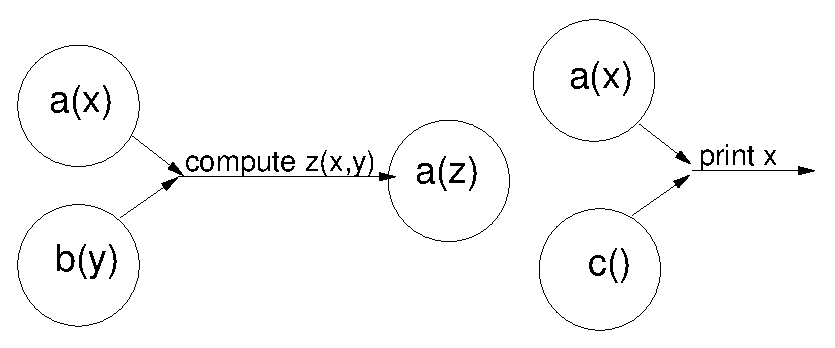
\includegraphics[width=1\columnwidth]{cham2}

\texttt{\textcolor{blue}{\scriptsize{def~ a(x) \& b(y) =}}}{\scriptsize \par}

\texttt{\textcolor{blue}{\scriptsize{~ let z = (big\_function x y)
in a(z)}}}{\scriptsize \par}

\texttt{\textcolor{blue}{\scriptsize{and~ a(x) \& c() = (print\_int
x; 0);;}}}%
\end{minipage}\hfill{}\\
~\\
When reaction starts: input molecules disappear, expression is computed,
output molecules are injected


\lyxframeend{}


\lyxframeend{}\lyxframe{Join Calculus in a nutshell}


\framesubtitle{More features of JoCaml}
\begin{itemize}
\item Mutual recursion:\\
\texttt{\textcolor{blue}{\scriptsize{def a(x) = a(x+1) \& b(x+2) and
b(x) \& c(y) = a(x+y)}}}{\scriptsize \par}
\item Pattern-matching on molecule's payload values:\\
\texttt{\textcolor{blue}{\scriptsize{def a(Some x) \& b(y) = b(x+y)
or a(None) \& b(y) = b(y)}}}{\scriptsize \par}
\item \textbf{Instant} molecules (same type as function calls):\\
\texttt{\textcolor{blue}{\scriptsize{def a(x) \& f() = a(x+1) \& reply
x to f}}}{\scriptsize \par}
\item \textbf{Local} molecules and reactions: \\
\texttt{\textcolor{blue}{\scriptsize{def c(n) = ( if n>0 then c(n-1)
else 0 ) in~ spawn c(10)}}}{\scriptsize \par}
\item Injection as side-effect: \texttt{\textcolor{blue}{\scriptsize{~
let x=3 in (spawn a(x); printf ``\%d\textbackslash{}n'' x)}}} 
\item \textbf{Molecule} \textbf{constructors} are defined as values and
can be manipulated:\\
\texttt{\textcolor{blue}{\scriptsize{\# def a(x) = Printf.printf ``\%d\textbackslash{}n''
x; 0;;}}}\\
\texttt{\textcolor{blue}{\scriptsize{val a : int Join.chan = <abstr>}}}\\
\texttt{\textcolor{blue}{\scriptsize{\# def b(m,y) = Printf.printf
``injecting m(\%d)\textbackslash{}n'' y; m(y);;}}}\\
\texttt{\textcolor{blue}{\scriptsize{val b: (int Join.chan {*} int)
Join.chan = <abstr>}}}\\

\end{itemize}

\lyxframeend{}


\lyxframeend{}\lyxframe{Join Calculus: Examples}


\framesubtitle{Options, Futures, and Map/Reduce}

Future with synchronous poll (``\texttt{\textcolor{blue}{\scriptsize{get}}}''):\\
\texttt{\textcolor{blue}{\scriptsize{\# def fut(f,x) = let res = f
x in finished(res)}}}\\
\texttt{\textcolor{blue}{\scriptsize{~ and get() \& finished(res)
= reply res to get;;}}}\\
\texttt{\textcolor{blue}{\scriptsize{val get : unit -> '\_a = <fun>}}}\\
\texttt{\textcolor{blue}{\scriptsize{val finished : '\_a Join.chan
= <abstr>}}}\\
\texttt{\textcolor{blue}{\scriptsize{val fut : (('a -> '\_b) {*} 'a)
Join.chan = <abstr>}}}{\scriptsize \par}

Future with synchronous callback:\\
\texttt{\textcolor{blue}{\scriptsize{def fut(f,x,c) = let res = f
x in ( c(res); finished(res) )}}}\\
\texttt{\textcolor{blue}{\scriptsize{~ and get() \& finished(res)
= reply res to get}}}{\scriptsize \par}

Future with asynchronous callback:\\
\texttt{\textcolor{blue}{\scriptsize{def fut(f,x,m) = let res = f
x in ( m(res) \& finished(res) )}}}\\
\texttt{\textcolor{blue}{\scriptsize{~ and get() \& finished(res)
= reply res to get}}}{\scriptsize \par}
\begin{itemize}
\item Exercise: implement a ``future with cancellable callback''
\end{itemize}

\lyxframeend{}


\lyxframeend{}\lyxframe{Join Calculus: Examples}


\framesubtitle{Options, Futures, and Map/Reduce}

Asynchronous counter:\\
\texttt{\textcolor{blue}{\scriptsize{\# def inc() \& c(n) = c(n+1) }}}{\scriptsize \par}

\texttt{\textcolor{blue}{\scriptsize{or get() \& c(n) = reply n to
get \& c(n);; }}}{\scriptsize \par}

\texttt{\textcolor{blue}{\scriptsize{val inc : unit Join.chan = <abstr> }}}{\scriptsize \par}

\texttt{\textcolor{blue}{\scriptsize{val get : unit -> int = <fun> }}}{\scriptsize \par}

\texttt{\textcolor{blue}{\scriptsize{val c : int Join.chan = <abstr> }}}{\scriptsize \par}

\texttt{\textcolor{blue}{\scriptsize{\# spawn c(0) \& inc() \& inc()
\& inc();; }}}{\scriptsize \par}

\texttt{\textcolor{blue}{\scriptsize{- : unit = () }}}{\scriptsize \par}

\texttt{\textcolor{blue}{\scriptsize{\# get();; }}}{\scriptsize \par}

\texttt{\textcolor{blue}{\scriptsize{- : int = 3 }}}{\scriptsize \par}

Map/Reduce:\\
\texttt{\textcolor{blue}{\scriptsize{def res(list) \& c(s) = res (s::list)
or get() \& res(list) = reply list to get;;}}}\\
\texttt{\textcolor{blue}{\scriptsize{spawn res({[}{]});;}}} \\
\texttt{\textcolor{blue}{\scriptsize{List.map (fun x-> spawn c(x{*}2))
{[}1; 2; 3{]};;}}}\\
\texttt{\textcolor{blue}{\scriptsize{get();; ({*} this returned {[}4;
6; 2{]} in one test {*})}}}{\scriptsize \par}
\begin{itemize}
\item Exercise: implement a concurrent ``fold'' (e.g. sum of int list)
\end{itemize}

\lyxframeend{}


\lyxframeend{}\lyxframe{Join Calculus: Examples}


\framesubtitle{Five Dining Philosophers}

Philosophers \textcolor{blue}{\scriptsize{A}}\texttt{\textcolor{blue}{\scriptsize{,
}}}\textcolor{blue}{\scriptsize{B}}\texttt{\textcolor{blue}{\scriptsize{,
}}}\textcolor{blue}{\scriptsize{C}}\texttt{\textcolor{blue}{\scriptsize{,
}}}\textcolor{blue}{\scriptsize{D}}\texttt{\textcolor{blue}{\scriptsize{,
}}}\textcolor{blue}{\scriptsize{E}}; forks \texttt{\textcolor{blue}{\scriptsize{fAB,
fBC, fCD, fDE, fEA}}}.
\begin{lyxcode}
\textcolor{blue}{\scriptsize{let~report(message)~=~Printf.printf~``\%s\textbackslash{}n''~message;}}{\scriptsize \par}

\textcolor{blue}{\scriptsize{~~~~~~~~~~~~~~~~~~~~~~~~~~~Unix.sleep~(Random.int~3600)~;;}}{\scriptsize \par}

\textcolor{blue}{\scriptsize{def~hA()~\&~fEA()~\&~fAB()~=~report(``A~is~eating'');~tA()~\&~fEA()~\&~fAB()~}}{\scriptsize \par}

\textcolor{blue}{\scriptsize{or~~hB()~\&~fAB()~\&~fBC()~=~report(``B~is~eating'');~tB()~\&~fAB()~\&~fBC()~}}{\scriptsize \par}

\textcolor{blue}{\scriptsize{or~~hC()~\&~fBC()~\&~fCD()~=~report(``C~is~eating'');~tC()~\&~fBC()~\&~fCD()~}}{\scriptsize \par}

\textcolor{blue}{\scriptsize{or~~hD()~\&~fCD()~\&~fDE()~=~report(``D~is~eating'');~tD()~\&~fCD()~\&~fDE()~}}{\scriptsize \par}

\textcolor{blue}{\scriptsize{or~~hE()~\&~fDE()~\&~fEA()~=~report(``E~is~eating'');~tE()~\&~fDE()~\&~fEA()~}}{\scriptsize \par}

\textcolor{blue}{\scriptsize{and~tA()~=~report(``A~is~thinking'');~hA()~}}{\scriptsize \par}

\textcolor{blue}{\scriptsize{and~tB()~=~report(``B~is~thinking'');~hB()~}}{\scriptsize \par}

\textcolor{blue}{\scriptsize{and~tC()~=~report(``C~is~thinking'');~hC()~}}{\scriptsize \par}

\textcolor{blue}{\scriptsize{and~tD()~=~report(``D~is~thinking'');~hD()~}}{\scriptsize \par}

\textcolor{blue}{\scriptsize{and~tE()~=~report(``E~is~thinking'');~hE()~;;~}}{\scriptsize \par}



\textcolor{blue}{\scriptsize{spawn~fAB()~\&~fBC()~\&~fCD()~\&~fDE()~\&~fEA()}}{\scriptsize \par}

\textcolor{blue}{\scriptsize{~~~~~\&~tA()~\&~tB()~\&~tC()~\&~tD()~\&~tE()~;;~}}{\scriptsize \par}
\end{lyxcode}

\lyxframeend{}


\lyxframeend{}\lyxframe{Limitations and restrictions of Join Calculus}


\framesubtitle{Less is more!}
\begin{itemize}
\item Reactions are defined \textbf{statically} and with \textbf{local scope}:

\begin{itemize}
\item no molecules with computed names: \texttt{\textcolor{blue}{\scriptsize{}}}~\\
\texttt{\textcolor{blue}{\scriptsize{a(x) \& molecule\_named(``b'')(x)
= (not allowed!)}}}{\scriptsize \par}
\item cannot dynamically add a new reaction to a previously defined molecule:\texttt{\textcolor{blue}{\scriptsize{}}}~\\
\texttt{\textcolor{blue}{\scriptsize{def a(x) \& b(y) = ... ;;}}}~\\
\texttt{\textcolor{blue}{\scriptsize{def b(y) \& c(z) = ... shadows
the old definition of b()!}}}{\scriptsize \par}
\end{itemize}
\item No ``guard conditions'' for reactions:
\end{itemize}
\texttt{\textcolor{blue}{\scriptsize{def a(x) \& b(y) \& start\_if
(x==y) = ... (not allowed!)}}}{\scriptsize \par}
\begin{itemize}
\item No duplicated input values: \texttt{\textcolor{blue}{\scriptsize{a(x)
\& b(x) = (not allowed!)}}}{\scriptsize \par}
\item No duplicated input molecules: \texttt{\textcolor{blue}{\scriptsize{a(x)
\& a(y) = (not allowed!)}}}{\scriptsize \par}
\item No way to test dynamically for the presence/absence of a molecule!
\end{itemize}
\texttt{\textcolor{blue}{\scriptsize{def a(x) \& b(y) = if have\_molecules(c
\& d) then ... else ... (not allowed!)}}}{\scriptsize \par}


\lyxframeend{}


\lyxframeend{}\lyxframe{Limitations and restrictions of Join Calculus}


\framesubtitle{It seems they do not limit the expressive power!}

What if we \emph{need} a reaction with pairs of molecules?

\texttt{\textcolor{blue}{\scriptsize{a(x) \& a(y) = a(x+y) }}}{\scriptsize \par}
\begin{itemize}
\item Solution: use two \textquotedbl{}\texttt{\textcolor{blue}{\scriptsize{or}}}\textquotedbl{}-coupled
reactions with new molecules \texttt{\textcolor{blue}{\scriptsize{a'}}}
and \texttt{\textcolor{blue}{\scriptsize{b}}}:
\end{itemize}
\texttt{\textcolor{blue}{\scriptsize{def a(x) \& b() = a'(x) or a(x)
\& a'(y) = whatever(x,y) }}}{\scriptsize \par}
\begin{itemize}
\item Make sure that one \texttt{\textcolor{blue}{\scriptsize{b()}}} is
injected together with each \texttt{\textcolor{blue}{\scriptsize{a(x)}}}{\scriptsize \par}
\end{itemize}
Questions:
\begin{itemize}
\item Can we prevent the error of not injecting \texttt{\textcolor{blue}{\scriptsize{b()}}}?
\item Can we do a reaction with $n$ molecules, where $n$ is dynamic?
\item Can we do ``$n$ dining philosophers''?
\end{itemize}

\lyxframeend{}


\lyxframeend{}\lyxframe{Local scope and recursion}


\framesubtitle{Skeleton code for concurrent merge-sort}

The \texttt{mergesort} molecule:
\begin{itemize}
\item receives the upper-level ``\texttt{\textcolor{blue}{\scriptsize{sorted\_result}}}''
molecule
\item defines its own ``\texttt{\textcolor{blue}{\scriptsize{sorted}}}''
molecule in \emph{local scope}
\item emits upper-level ``\texttt{\textcolor{blue}{\scriptsize{sorted\_result}}}''
when done\end{itemize}
\begin{lyxcode}
\textcolor{blue}{\scriptsize{def~mergesort(arr,~sorted\_result)~=~}}{\scriptsize \par}

\textcolor{blue}{\scriptsize{~~if~Array.length~arr~<=~1~then~sorted\_result(arr)}}{\scriptsize \par}

\textcolor{blue}{\scriptsize{~~else~}}{\scriptsize \par}

\textcolor{blue}{\scriptsize{~~~let~(part1,~part2)~=~array\_split~arr}}{\scriptsize \par}

\textcolor{blue}{\scriptsize{~~~in~}}{\scriptsize \par}

\textcolor{blue}{\scriptsize{~~~def~sorted(x)~\&~sorted'(y)~=~sorted\_result(array\_merge~x~y)~}}{\scriptsize \par}

\textcolor{blue}{\scriptsize{~~~in~}}{\scriptsize \par}

\textcolor{blue}{\scriptsize{~~~mergesort(part1,~sorted)~\&~mergesort(part2,~sorted')}}{\scriptsize \par}
\end{lyxcode}
Note  ``\texttt{\textcolor{blue}{\scriptsize{sorted(x) \& sorted'(y)}}}'':
need different molecules.

See tutorial for complete working JoCaml code.


\lyxframeend{}


\lyxframeend{}\lyxframe{Comparison: Join Calculus vs. Actor model}

Reaction $\approx$ actor; molecule $\approx$ message to actor.

Actors: 
\begin{itemize}
\item need to be created and started explicitly
\item process one message at a time (one actor = one thread)
\item must hold mutable state (e.g. for a thread-safe counter)
\item explicitly create and configure other actors 
\end{itemize}
Reactions:
\begin{itemize}
\item start when several molecules are available
\item many reactions can start at once, automatically
\item do not need mutable state
\item all reactions are defined statically, but locally scoped
\item simulate actors:\textcolor{blue}{\scriptsize{ def message(m) \& actor(state)
= actor(compute\_new state m)}}{\scriptsize \par}
\end{itemize}

\lyxframeend{}


\lyxframeend{}\lyxframe{Implementation of Join Calculus}


\framesubtitle{JC = a DSL + run-time library, or just DSL?}

Implement Join Calculus using Actors (Akka)?
\begin{itemize}
\item Each reaction has $1$ ``monitor actor'' and $\geq1$ ``worker
actors''
\item Monitor receives messages for each ``spawn'', keeps track of molecules
\item Monitor starts a worker actor when all molecules are present
\item Monitors have to talk to competing monitors - ``use up'' molecules

\begin{itemize}
\item but all competitions are statically defined!
\end{itemize}
\item Monitors / workers need to be locally scoped!
\item No globally shared state of the ``soup'' is needed!
\item Discuss
\end{itemize}

\lyxframeend{}


\lyxframeend{}\lyxframe{Conclusions and outlook}
\begin{itemize}
\item ``Join Calculus'' is concurrent programming in pure functional style
\item Similar to ``Actors'', but more concurrent and ``more pure''
\item Very little known, and very little used in practice
\item Existing literature is not suitable as introduction to practical programming
\item My tutorial text is in progress (search Google for ``tutorial on
join calculus'')
\end{itemize}

\lyxframeend{}
\end{document}
